% This file was created by matlab2tikz.
%
%The latest updates can be retrieved from
%  http://www.mathworks.com/matlabcentral/fileexchange/22022-matlab2tikz-matlab2tikz
%where you can also make suggestions and rate matlab2tikz.
%
\definecolor{mycolor1}{rgb}{0.00000,0.44700,0.74100}%
%
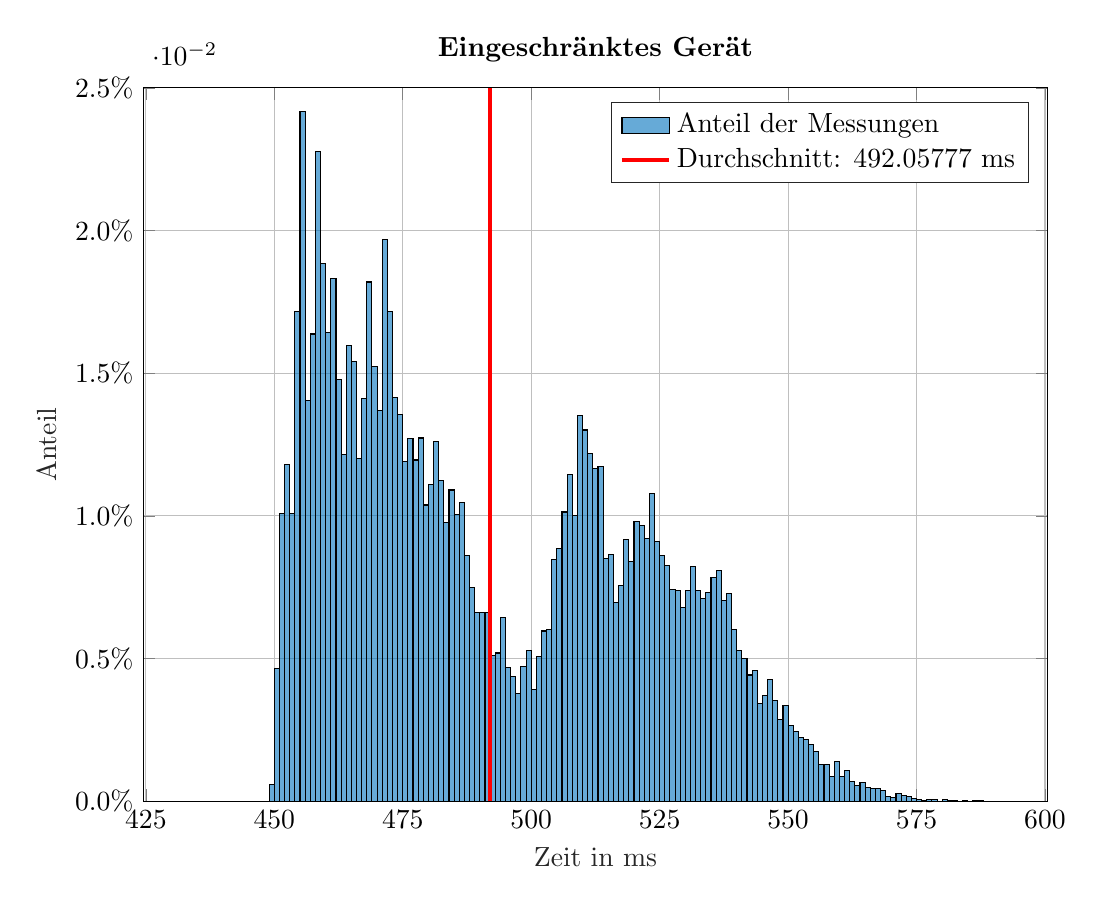
\begin{tikzpicture}

\begin{axis}[%
width=4.521in,
height=3.566in,
at={(0.758in,0.481in)},
scale only axis,
xmin=424.5,
xmax=600.5,
xtick={425, 450, 475, 500, 525, 550, 575, 600},
xlabel style={font=\color{white!15!black}},
xlabel={Zeit in ms},
ymin=0,
ymax=0.025,
ytick={0,0.005,0.01,0.015,0.02,0.025},
yticklabels={{0.0\%},{0.5\%},{1.0\%},{1.5\%},{2.0\%},{2.5\%}},
ylabel style={font=\color{white!15!black}},
ylabel={Anteil},
axis background/.style={fill=white},
title style={font=\bfseries},
title={Eingeschr{\"a}nktes Ger{\"a}t},
xmajorgrids,
ymajorgrids,
legend style={legend cell align=left, align=left, draw=white!15!black}
]
\addplot[ybar interval, fill=mycolor1, fill opacity=0.6, draw=black, area legend] table[row sep=crcr] {%
x	y\\
449	0.000586963237565647\\
450	0.0046339202965709\\
451	0.0100710534445474\\
452	0.0118010503552672\\
453	0.0100710534445474\\
454	0.0171763978992895\\
455	0.024158171146123\\
456	0.0140562248995984\\
457	0.0163731850478838\\
458	0.0227679950571517\\
459	0.018844609206055\\
460	0.0164349706518381\\
461	0.0183194315724436\\
462	0.0147667593450726\\
463	0.0121408711770158\\
464	0.015971578622181\\
465	0.0154155081865925\\
466	0.0120172999691072\\
467	0.0141180105035527\\
468	0.0181958603645351\\
469	0.0152301513747297\\
470	0.0136855112758727\\
471	0.0196787148594378\\
472	0.0171763978992895\\
473	0.0141489033055298\\
474	0.0135619400679642\\
475	0.0118937287611986\\
476	0.0126969416126043\\
477	0.0119555143651529\\
478	0.0127278344145814\\
479	0.0103799814643188\\
480	0.011090515909793\\
481	0.0126042632066728\\
482	0.0112449799196787\\
483	0.00976212542477603\\
484	0.0109051590979302\\
485	0.0100401606425703\\
486	0.0104726598702502\\
487	0.00861909175162187\\
488	0.00747605807846772\\
489	0.00661105962310782\\
490	0.00661105962310782\\
491	0.00661105962310782\\
492	0.00509731232622799\\
493	0.00518999073215941\\
494	0.00642570281124498\\
495	0.00469570590052518\\
496	0.00435588507877665\\
497	0.003768921841211\\
498	0.00472659870250232\\
499	0.00528266913809082\\
500	0.00392338585109669\\
501	0.00506641952425085\\
502	0.00596231078158789\\
503	0.00602409638554217\\
504	0.00846462774173617\\
505	0.00886623416743899\\
506	0.0101328390485017\\
507	0.0114612295335187\\
508	0.0100092678405931\\
509	0.013531047265987\\
510	0.0130058696323757\\
511	0.0121717639789929\\
512	0.0116465863453815\\
513	0.0117392647513129\\
514	0.00849552054371332\\
515	0.00864998455359901\\
516	0.00695088044485635\\
517	0.00756873648439913\\
518	0.00917516218721038\\
519	0.0084028421377819\\
520	0.00979301822675317\\
521	0.00966944701884461\\
522	0.00920605498918752\\
523	0.0107815878900216\\
524	0.0091133765832561\\
525	0.00861909175162187\\
526	0.0082483781278962\\
527	0.00741427247451344\\
528	0.0073833796725363\\
529	0.00679641643497065\\
530	0.0073833796725363\\
531	0.00821748532591906\\
532	0.0073833796725363\\
533	0.00710534445474204\\
534	0.00732159406858202\\
535	0.00784677170219339\\
536	0.0080939141180105\\
537	0.00704355885078777\\
538	0.00729070126660488\\
539	0.00602409638554217\\
540	0.00528266913809082\\
541	0.00500463392029657\\
542	0.00441767068273092\\
543	0.00457213469261662\\
544	0.00342910101946247\\
545	0.00370713623725672\\
546	0.00426320667284523\\
547	0.00352177942539388\\
548	0.00287303058387396\\
549	0.00333642261353105\\
550	0.00265678097003398\\
551	0.00244053135619401\\
552	0.00222428174235403\\
553	0.00216249613839975\\
554	0.00197713932653692\\
555	0.0017299969107198\\
556	0.00126660488106271\\
557	0.00129749768303985\\
558	0.000864998455359901\\
559	0.00139017608897127\\
560	0.000864998455359901\\
561	0.00108124806919988\\
562	0.000679641643497065\\
563	0.000556070435588508\\
564	0.000648748841519926\\
565	0.00046339202965709\\
566	0.000432499227679951\\
567	0.000432499227679951\\
568	0.000370713623725672\\
569	0.000154464009885697\\
570	0.000123571207908557\\
571	0.000278035217794254\\
572	0.000185356811862836\\
573	0.000154464009885697\\
574	9.2678405931418e-05\\
575	6.17856039542787e-05\\
576	3.08928019771393e-05\\
577	6.17856039542787e-05\\
578	6.17856039542787e-05\\
579	0\\
580	6.17856039542787e-05\\
581	3.08928019771393e-05\\
582	3.08928019771393e-05\\
583	0\\
584	3.08928019771393e-05\\
585	0\\
586	3.08928019771393e-05\\
587	3.08928019771393e-05\\
588	3.08928019771393e-05\\
};
\addlegendentry{Anteil der Messungen}

\addplot [color=red, line width=1.5pt]
  table[row sep=crcr]{%
492.057769539697	0\\
492.057769539697	0.025\\
};
\addlegendentry{Durchschnitt: 492.05777 ms}

\end{axis}
\end{tikzpicture}%